\documentclass[aspectratio=1610,onlymath]{beamer}
% \documentclass[aspectratio=1610,onlymath,handout]{beamer}

\input{macros-lecture}

\defineTitle{16}{Logisches Schließen (2)}{21. Juni 2021}

\begin{document}

\maketitle

\begin{frame}\frametitle{Schließen ist schwer}

\emph{Erinnerung:} $F$ ist logische Konsequenz von $G$, wenn alle Modelle von $F$ auch Modelle von $G$ sind.
\begin{itemize}
\item Es ist nicht offensichtlich, wie man das überprüfen sollte, denn es gibt unendlich viele Modelle
\item Ebenso schwer erscheinen die gleichwertigen Probleme der Erfüllbarkeit und Allgemeingültigkeit
\end{itemize}\pause
\emph{Intuition:} prädikatenlogisches Schließen ist unentscheidbar
\bigskip

\alert{Wie kann man das beweisen?}\pause\bigskip

Durch Reduktion eines bekannten unentscheidbaren Problems, \ghost{z.B.}
\begin{itemize}
\item Halteproblem
\item Postsches Korrespondenzproblem
\item Äquivalenz kontextfreier Sprachen
\item \ldots
\end{itemize}

\end{frame}


\begin{frame}\frametitle{Unentscheidbarkeit (1)}

\theobox{\emph{Satz:} Logisches Schließen (Erfüllbarkeit, Allgemeingültigkeit, logische Konsequenz) in der Prädikatenlogik ist unentscheidbar.}

\emph{Beweis:} Durch Reduktion vom CFG-Schnittproblem:\smallskip

~~~~~\emph{Gegeben:} Kontextfreie Grammatiken $G_1$ und $G_2$\\
~~~~~\emph{Frage:} Gibt es ein Wort $w\in\Slang{L}(G_1)\cap\Slang{L}(G_2)$?
\bigskip\pause

\emph{Idee:} Wir kodieren Wörter in der Prädikatenlogik als
Ketten von binären Relationen.\medskip\pause

Zum Beispiel würde das Wort $\Sterm{russell}$ in einer Modellstruktur $\Inter$
wie folgt aussehen:

\begin{center}
\scalebox{1.0}{%
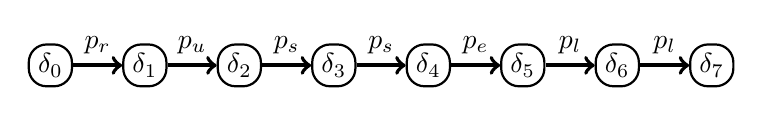
\begin{tikzpicture}[scale=1.2]
% \draw[help lines] (0,0) grid (7,2);

\node (d0) [rectangle,rounded corners=1.5ex, minimum width=1.5em, minimum height=1.5em, draw=black,thick] at (0,0) {$\delta_0$};
\node (d1) [rectangle,rounded corners=1.5ex, minimum width=1.5em, minimum height=1.5em, draw=black,thick] at (1,0) {$\delta_1$};
\node (d2) [rectangle,rounded corners=1.5ex, minimum width=1.5em, minimum height=1.5em, draw=black,thick] at (2,0) {$\delta_2$};
\node (d3) [rectangle,rounded corners=1.5ex, minimum width=1.5em, minimum height=1.5em, draw=black,thick] at (3,0) {$\delta_3$};
\node (d4) [rectangle,rounded corners=1.5ex, minimum width=1.5em, minimum height=1.5em, draw=black,thick] at (4,0) {$\delta_4$};
\node (d5) [rectangle,rounded corners=1.5ex, minimum width=1.5em, minimum height=1.5em, draw=black,thick] at (5,0) {$\delta_5$};
\node (d6) [rectangle,rounded corners=1.5ex, minimum width=1.5em, minimum height=1.5em, draw=black,thick] at (6,0) {$\delta_6$};
\node (d7) [rectangle,rounded corners=1.5ex, minimum width=1.5em, minimum height=1.5em, draw=black,thick] at (7,0) {$\delta_7$};

\path[->,line width=0.5mm](d0) edge node[above] {$p_{\Sterm{r}}$} (d1);
\path[->,line width=0.5mm](d1) edge node[above] {$p_{\Sterm{u}}$} (d2);
\path[->,line width=0.5mm](d2) edge node[above] {$p_{\Sterm{s}}$} (d3);
\path[->,line width=0.5mm](d3) edge node[above] {$p_{\Sterm{s}}$} (d4);
\path[->,line width=0.5mm](d4) edge node[above] {$p_{\Sterm{e}}$} (d5);
\path[->,line width=0.5mm](d5) edge node[above] {$p_{\Sterm{l}}$} (d6);
\path[->,line width=0.5mm](d6) edge node[above] {$p_{\Sterm{l}}$} (d7);

\end{tikzpicture}}
\end{center}

Diese Skizze soll bedeuten, dass z.B. $\tuple{\delta_2,\delta_3},\tuple{\delta_3,\delta_4}\in p_{\Sterm{s}}^\Inter$.
Wir verwenden ein Prädikatensymbol $p_{\Sterm{a}}$ für jedes Alphabetssymbol ${\Sterm{a}}$.

\end{frame}


\begin{frame}\frametitle{Unentscheidbarkeit (2)}

\theobox{\emph{Satz:} Logisches Schließen (Erfüllbarkeit, Allgemeingültigkeit, logische Konsequenz) in der Prädikatenlogik ist unentscheidbar.}

\emph{Beweis (Fortsetzung):} Zusätzlich verwenden wir binäre Prädikatensymbole
$p_{\Snterm{A}}$ für jedes Nichtterminalsymbol $\Snterm{A}$.
\bigskip\pause

Die Kodierung von Grammatiken ist nun direkt möglich:
\begin{itemize}
\item Wir nehmen o.B.d.A. an, dass $G_1$ und $G_2$ keine Nichtterminale gemeinsam haben.
\item Eine Produktionsregel $\Snterm{A}\to \sigma_1\cdots\sigma_n$ kodieren wir als Formel:
\[ \forall x_0,\ldots,x_n. \big((p_{\sigma_1}(x_0,x_1)\wedge \ldots\wedge p_{\sigma_n}(x_{n-1},x_n)) \to p_{\Snterm{A}}(x_0,x_n)\big)\]
\item Idee: die Formel \alert{erkennt}, ob eine gegebene Kette aus Terminalen und Nichtterminalen aus einem anderen Nichtterminal entstehen kann
\end{itemize}

\end{frame}


\begin{frame}\frametitle{Unentscheidbarkeit (3)}

\theobox{\emph{Satz:} Logisches Schließen (Erfüllbarkeit, Allgemeingültigkeit, logische Konsequenz) in der Prädikatenlogik ist unentscheidbar.}

\emph{Beweis (Fortsetzung):} Seien $\Sntermsub{S}{1}$ und $\Sntermsub{S}{2}$ die Startsymbole von $G_1$ und $G_2$.
Dann wollen wir das Schnittproblem kodieren, indem wir fragen, ob die folgende Formel folgt:\\[1ex]
\narrowcentering{$ \exists x,y. (p_{\Sntermsub{S}{1}}(x,y)\wedge p_{\Sntermsub{S}{2}}(x,y))$}\\[1ex]

Was fehlt?\pause
\begin{itemize}
\item Die Grammatik-Formeln können erkennen, ob eine Zeichenkette aus $\Sntermsub{S}{1}$ oder $\Sntermsub{S}{2}$ abgeleitet werden kann
\item Jede Interpretation, welche die Kodierung eines Wortes $w\in\Slang{L}(G_1)\cap\Slang{L}(G_2)$ enthält, muss daher auch die Formel $\exists x,y. (p_{\Sntermsub{S}{1}}(x,y)\wedge p_{\Sntermsub{S}{2}}(x,y))$ erfüllen
\item Aber: Es kann auch Interpretationen geben, welche keine Kodierung von $w$ enthalten
\end{itemize}
$\leadsto$ Alle möglichen Wörter müssten kodiert vorkommen \ldots
\end{frame}

\begin{frame}\frametitle{Unentscheidbarkeit (4)}

\theobox{\emph{Satz:} Logisches Schließen (Erfüllbarkeit, Allgemeingültigkeit, logische Konsequenz) in der Prädikatenlogik ist unentscheidbar.}

\emph{Beweis (Fortsetzung):} Alle möglichen Wörter müssten kodiert vorkommen \ldots{}
% \bigskip
Dazu fügen wir noch folgende Sätze hinzu:
\[ \forall x.\exists y.p_{\Sterm{a}}(x,y) \qquad \text{für jedes Terminalsymbol $\Sterm{a}$}\]\pause\vspace{-7mm}

\begin{itemize}
\item Jedes Modell dieser Theorie muss Kodierungen aller Wörter enthalten (aber eventuell als zyklische oder überlappende Pfade, z.B. in einem Modell mit nur einem Element, welches in jeder möglichen Relation zu sich selbst steht)\pause
\item Gibt es ein Wort $w\in\Slang{L}(G_1)\cap\Slang{L}(G_2)$, dann muss auch dieses Wort kodiert vorkommen: es folgt $ \exists x,y. (p_{\Sntermsub{S}{1}}(x,y)\wedge p_{\Sntermsub{S}{2}}(x,y))$\pause
\item Folgt $\exists x,y. (p_{\Sntermsub{S}{1}}(x,y)\wedge p_{\Sntermsub{S}{2}}(x,y))$, erfüllen alle Modelle diesen Satz, speziell auch das Modell, welches man erhält, indem man einen unendlichen Baum aller Wörter aufbaut
\end{itemize}


\end{frame}

\begin{frame}\frametitle{Unentscheidbarkeit (5)}

\theobox{\emph{Satz:} Logisches Schließen (Erfüllbarkeit, Allgemeingültigkeit, logische Konsequenz) in der Prädikatenlogik ist unentscheidbar.}

\emph{Beweis (Fortsetzung):} Skizze des "`kanonischen"' baumförmigen Modells, welches keine Zyklen oder parallelen Relationen enthält, über Alphabet $\{\Sterm{a},\Sterm{b}\}$ (ohne eventuelle Kanten für Nichtterminale):

\begin{center}
\scalebox{1.0}{%
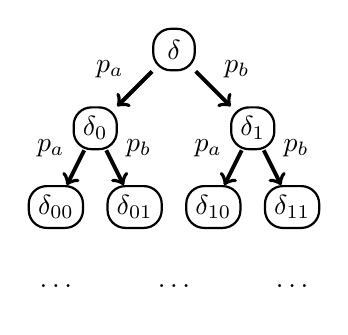
\begin{tikzpicture}[scale=1]
% \draw[help lines] (0,0) grid (7,2);

\node (d) [rectangle,rounded corners=1.5ex, minimum width=1.5em, minimum height=1.5em, draw=black,thick] at (0,0) {$\delta$};
\node (d0) [rectangle,rounded corners=1.5ex, minimum width=1.5em, minimum height=1.5em, draw=black,thick] at (-1,-1) {$\delta_0$};
\node (d1) [rectangle,rounded corners=1.5ex, minimum width=1.5em, minimum height=1.5em, draw=black,thick] at (1,-1) {$\delta_1$};

\node (d00) [rectangle,rounded corners=1.5ex, minimum width=1.5em, minimum height=1.5em, draw=black,thick] at (-1.5,-2) {$\delta_{00}$};
\node (d01) [rectangle,rounded corners=1.5ex, minimum width=1.5em, minimum height=1.5em, draw=black,thick] at (-0.5,-2) {$\delta_{01}$};
\node (d10) [rectangle,rounded corners=1.5ex, minimum width=1.5em, minimum height=1.5em, draw=black,thick] at (0.5,-2) {$\delta_{10}$};
\node (d11) [rectangle,rounded corners=1.5ex, minimum width=1.5em, minimum height=1.5em, draw=black,thick] at (1.5,-2) {$\delta_{11}$};

\path[->,line width=0.5mm](d) edge node[above left] {$p_{\Sterm{a}}$} (d0);
\path[->,line width=0.5mm](d) edge node[above right] {$p_{\Sterm{b}}$} (d1);
\path[->,line width=0.5mm](d0) edge node[above left] {$p_{\Sterm{a}}$} (d00);
\path[->,line width=0.5mm](d0) edge node[above right] {$p_{\Sterm{b}}$} (d01);
\path[->,line width=0.5mm](d1) edge node[above left] {$p_{\Sterm{a}}$} (d10);
\path[->,line width=0.5mm](d1) edge node[above right] {$p_{\Sterm{b}}$} (d11);

\node (e1) [rectangle,rounded corners=1.5ex, minimum width=1.5em, minimum height=1.5em, draw=none,thick] at (-1.5,-3) {$\ldots$};
\node (e2) [rectangle,rounded corners=1.5ex, minimum width=1.5em, minimum height=1.5em, draw=none,thick] at (0,-3) {$\ldots$};
\node (e3) [rectangle,rounded corners=1.5ex, minimum width=1.5em, minimum height=1.5em, draw=none,thick] at (1.5,-3) {$\ldots$};

\end{tikzpicture}}
\end{center}

Falls "`sogar"' dieses Modell $ \exists x,y. (p_{\Sntermsub{S}{1}}(x,y)\wedge p_{\Sntermsub{S}{2}}(x,y))$ erfüllt, dann muss es ein Wort $w\in\Slang{L}(G_1)\cap\Slang{L}(G_2)$ geben.


\end{frame}

\begin{frame}\frametitle{Unentscheidbarkeit (6)}

\theobox{\emph{Satz:} Logisches Schließen (Erfüllbarkeit, Allgemeingültigkeit, logische Konsequenz) in der Prädikatenlogik ist unentscheidbar.}

\emph{Beweis (Zusammenfassung):} Wir konstruieren aus $G_1$ und $G_2$ eine logische Theorie $\mathcal{T}$ mit den folgenden Sätzen:
\begin{itemize}
\item für jede Produktionsregel $\Snterm{A}\to \sigma_1\cdots\sigma_n$ von $G_1$ oder $G_2$:
\[\forall x_0,\ldots,x_n. \big((p_{\sigma_1}(x_0,x_1)\wedge \ldots\wedge p_{\sigma_n}(x_{n-1},x_n)) \to p_{\Snterm{A}}(x_0,x_n)\big)\]
\item Für jedes Terminalsymbol $\Sterm{a}$:
\[\forall x.\exists y. p_{\Sterm{a}}(x,y)\]
\end{itemize}
Dann gilt $\mathcal{T}\models\exists x,y. (p_{\Sntermsub{S}{1}}(x,y)\wedge p_{\Sntermsub{S}{2}}(x,y))$ genau dann wenn es ein Wort $w\in\Slang{L}(G_1)\cap\Slang{L}(G_2)$ gibt.
\bigskip

Die Unentscheidbarkeit von Erfüllbarkeit und Allgemeingültigkeit folgt, weil man logische Konsequenz auf diese Probleme reduzieren kann.
\qed

\end{frame}


\begin{frame}\frametitle{Einfache Folgerungen}

Offensichtlich wird das Schließen nicht einfacher, wenn man auch noch Gleichheit erlaubt:\bigskip

\theobox{\emph{Korollar:} Logisches Schließen (Erfüllbarkeit, Allgemeingültigkeit, logische Konsequenz) in der Prädikatenlogik mit Gleichheit ist unentscheidbar.}\bigskip

Umgekehrt kann man aus dem Beweis noch stärkere Ergebnisse folgern, z.B.:

\theobox{\emph{Korollar:} Logisches Schließen (Erfüllbarkeit, Allgemeingültigkeit, logische Konsequenz) in der Prädikatenlogik ist unentscheidbar, selbst dann, wenn nur binäre Prädikatssymbole verwendet werden.}\bigskip

\end{frame}

\begin{frame}\frametitle{Unentscheidbarkeit hat viele Beweise}

Unser Unentscheidbarkeitsbeweis ist nicht der Einzige \ldots
\begin{itemize}
\item Mit Prädikatenlogik kann man viele mathematische Definitionen
direkt ausdrücken
\item Viele Probleme lassen sich dadurch ziemlich einfach kodieren
\item Der erste Schritt ist am wichtigsten:\\
	Wie wollen wir das Problem in logischen Interpretationen mit Relationen darstellen?
\item Sind die Prädikatensymbole einmal festgelegt, dann muss man nur noch
die Problemdefinition in diese Kodierung übersetzen.
\end{itemize}\pause

\examplebox{\emph{Beispiel:} Wir könnten das Halteproblem von TMs direkt kodieren, aber
dabei benötigt man viel mehr Prädikate. Es ist nicht schwer, Aussagen zu kodieren wie z.B. "`Falls es einen Zeitpunkt $t$ gibt, an dem die TM in Zustand $q$ an Position $y$ das Zeichen \Sterm{a} liest, dann folgt auf $t$ ein Zeitpunkt $t'$, an dem die TM in Zustand $q'$ ist."' Der Beweis ist leicht, sofern man keine relevante Aussage vergisst.}

\end{frame}

\frame{\label{frame_goedel}\begin{center}
\includegraphics[height=5cm]{images/Goedel.jpg}

\LARGE
Gödel
\end{center}}

\begin{frame}\frametitle{Zwischenstand}

Wir haben bisher zwei Dinge erkannt:
\begin{enumerate}[(1)]
\item \alert{Prädikatenlogik ist sehr ausdrucksstark:}
mit ihr können wir z.B. das mathematische Konzept der Gleichheit axiomatisieren oder
Probleme über formale Sprachen beschreiben
\item \alert{Prädikatenlogisches Schließen ist unentscheidbar:}
man kann Probleme definieren, die nicht mehr algorithmisch lösbar sind
\end{enumerate}

Eignet sich Prädikatenlogik also als universelle Beschreibungssprache für
die Mathematik (und darüber hinaus)?
\bigskip

Dazu hat Kurt Gödel (1906--1978) einiges zu sagen \ldots

\end{frame}

\begin{frame}\frametitle{Gödels Einsichten}

Gödel zeigte einige wesentliche Dinge:
\begin{enumerate}[(1)]
\item \alert{Gödelscher Vollständigkeitssatz (1930):}\\
"`Es gibt ein konsistentes Verfahren, das alle Konsequenzen einer prädikatenlogischen Theorie
effektiv beweisen kann."'
\begin{itemize}
\item Alle wahren Sätze können endlich bewiesen werden
\item Prädikatenlogisches Schließen ist semi-entscheidbar
\end{itemize}\pause
%
\item \alert{1. Gödelscher Unvollständigkeitssatz (1931):} \\
"`Es gibt kein konsistentes Verfahren, das alle Konsequenzen der elementaren Arithmetik
effektiv beweisen kann."'
\begin{itemize}
\item Für jedes Verfahren gibt es allgemeingültige Sätze über elementare arithmetische Zusammenhänge, die nicht bewiesen werden können
\item Die Wahrheit elementarer arithmetischer Zusammenhänge ist nicht semi-entscheidbar
\end{itemize}\pause
\item \alert{2. Gödelscher Unvollständigkeitssatz (1931):} später
\end{enumerate}

Mehr dazu in späteren Vorlesungen \ldots

\end{frame}

\sectionSlide{Algorithmen zum logischen Schließen}

\begin{frame}\frametitle{Wie können wir logisch Schließen?}

Gödel betrachtete ein konkretes Verfahren zum logischen Schließen,
basierend auf:
\begin{itemize}
\item einer Menge an vorgegebenen Tautologien
\item einer Menge von Regeln, mit denen man aus bereits bekannten Tautologien
neue ableiten kann
\end{itemize}
\alert{Diese Art von Verfahren war seit der Antike bekannt.}
\bigskip\pause

Gödel zeigte, dass dieses Verfahren die Semantik der Prädikatenlogik genau
einfängt:
\begin{itemize}
\item Das Verfahren ist \redalert{korrekt} (es leitet nur echte Tautologien ab) -- das war bekannt
\item Das Verfahren ist \redalert{vollständig} (es kann jede Tautologie auch irgendwie ableiten) -- ein Durchbruch, Gödels Vollständigkeitssatz
\end{itemize}

\end{frame}

\begin{frame}\frametitle{Theorie und Praxis}

Gödel zeigte damit auch die Semientscheidbarkeit des logischen Schließens:
\begin{itemize}
\item Man kann systematisch alle möglichen Ableitungen neuer Tautologien
bilden
\item Eine Formel ist eine Tautologie genau dann wenn sie irgendwann abgeleitet wird
\item Ist eine Formel keine Tautologie, dann werden wir es auf diese Art nie erfahren
\end{itemize}\pause

Das ist nicht sehr praktisch, wenn man wissen will, ob eine gegebene Formel $F$ eine
Tautologie ist \ldots
\bigskip

\alert{Geht es besser?}\pause
\begin{itemize}
\item Logisches Schließen ist unentscheidbar: kein Verfahren kann die Frage nach Allgemeingültigkeit sicher beantworten
\item Aber: Es gibt effizientere, zielgerichtetere Methoden
\end{itemize}

Für echte Implementierungen (Jahrzehnte später!) wurden bessere Algorithmen entwickelt

\end{frame}

\begin{frame}\frametitle{Bessere Algorithmen}\pause

Ein besonders erfolgreicher Algorithmus in praktischen Implementierungen ist
\redalert{Resolution}\bigskip\pause

\anybox{strongyellow}{
\emph{Rückblick:} Resolution in Aussagenlogik (Formale Systeme, V.23)%
\begin{itemize}
\item Methode zum Test auf Unerfüllbarkeit
\item Die Formel wird zunächst umgeformt in \redalert{Klauselform} (KNF) = konjunktive Normalform in Mengenschreibweise
\item In jedem Ableitungsschritt leitet man aus zwei zueinander passenden Klauseln eine neue ab:
\[  \frac{ \{L_1, \ldots, L_n, \alert{A}\}\qquad \{\alert{\neg A}, L'_1, \ldots, L'_m\}}{\{L_1, \ldots, L_n, L'_1, \ldots, L'_m\}} \]
\item Das Verfahren endet, wenn man entweder die \redalert{leere Klausel} erhält (unerfüllbar) oder, andernfalls, wenn keine neuen Klauseln mehr erzeugt werden können (erfüllbar)
\end{itemize}
}

\end{frame}

\begin{frame}\frametitle{Resolution in Prädikatenlogik}

Resolution in der Prädikatenlogik funktioniert ganz ähnlich:
\begin{enumerate}[(1)]
\item Umformung in Klauselform
\item Durchführung von Resolutionsschritten, bei denen jeweils zwei Klauseln kombiniert werden
\item Terminierung wenn leere Klausel auftritt oder keine neuen Klauseln mehr entstehen
\end{enumerate}
\bigskip

Wir müssen aber mehr beachten als zuvor:
\begin{itemize}
\item Die Umformung in Klauselform muss jetzt \alert{Quantoren} berücksichtigen
\item Die Resolutionsschritte müssen die \alert{kompliziertere Form von Atomen} (Prädikate mit Termen als Parameter) berücksichtigen
\item Es wird im Allgemeinen möglich sein, unendlich viele Klauseln abzuleiten ohne jemals die leere Klausel zu erzeugen -- \alert{Terminierung nicht garantiert}
\end{itemize}

\end{frame}

\sectionSlide{Syntaktische Umformungen in der Prädikatenlogik}

\begin{frame}\frametitle{Formeln umformen}

Wir haben bereits gelernt (Vorlesung 14):
\begin{itemize}
\item In prädikatenlogischen Formeln darf man Teilformeln durch semantisch äquivalente
Formeln ersetzen (Ersetzungstheorem)
\item Für die aussagenlogischen Junktoren gelten die gleichen Äquivalenzen wie in der Aussagenlogik
\end{itemize}
$\leadsto$ damit kann man schon viele Umformungen vornehmen
\bigskip

Es fehlen uns aber noch Äquivalenzen zum Umgang mit Quantoren

\end{frame}

\begin{frame}\frametitle{Äquivalenzen mit Quantoren}

Es gelten die folgenden Beziehungen:
\begin{align*}
\begin{split}
\neg\exists x.F &\equiv \forall x.\neg F\\
\neg\forall x.F &\equiv \exists x.\neg F
\end{split}
& \text{\textcolor{devilscss}{Negation von Quantoren}}\\[1ex]
%
\begin{split}
\exists x.\exists y.F &\equiv \exists y.\exists x.F\\
\forall x.\forall y.F &\equiv \forall y.\forall x.F
\end{split}
& \text{\textcolor{devilscss}{Kommutativität}}\\[1ex]
%
\exists x.(F\vee G) &\equiv (\exists x.F\vee \exists x.G) & \text{\textcolor{devilscss}{Distributivität $\exists$/$\vee$}}\\
\forall x.(F\wedge G) &\equiv (\forall x.F\wedge \forall x.G) & \text{\textcolor{devilscss}{Distributivität $\forall$/$\wedge$}}
\end{align*}

\pause\emph{Beweis:} Die Beweise ergeben sich direkt aus der Semantik, z.B.:\bigskip

\begin{tabular}{r@{ gdw. }l}
$\Inter,\Zuweisung\models \neg\exists x.F$
& $\Inter,\Zuweisung\not\models \exists x.F$\pause\\[-0.9ex]
& es gibt kein $\delta\in\Delta^\Inter$ mit $\Inter,\Zuweisung[x\mapsto\delta]\models F$\pause\\[-0.9ex]
& für alle $\delta\in\Delta^\Inter$ gilt $\Inter,\Zuweisung[x\mapsto\delta]\not\models F$\pause\\[-0.9ex]
& für alle $\delta\in\Delta^\Inter$ gilt $\Inter,\Zuweisung[x\mapsto\delta]\models \neg F$\pause\\[-0.9ex]
& $\Inter,\Zuweisung\models \forall x.\neg F$\hspace{4cm}~\qed
\end{tabular}

\end{frame}

\begin{frame}\frametitle{Nicht-Äquivalenzen mit Quantoren}

Andere ähnliche Beziehungen gelten \redalert{nicht}.\bigskip\pause

Es gilt \redalert{nicht} $\exists x.\forall y.F \equiv \forall y.\exists x.F$!\medskip

\examplebox{Zum Beispiel bedeutet $\forall x.\exists y.\textsf{hatVater}(x,y)$ "`Jeder hat einen Vater"' dagegen $\exists y.\forall x.\textsf{hatVater}(x,y)$ "`Jemand ist Vater aller."'\\[1ex]
{\tiny (Anmerkung: Gödel war übrigens religiös und hat einen philosophischen Gottesbeweis in modaler Logik formalisiert [siehe "`\href{https://en.wikipedia.org/wiki/G\%C3\%B6del\%27s_ontological_proof}{Gödel's ontological proof}"']; Russell war engagierter Atheist und scharfer Kritiker der Kirchen [siehe z.B. "`\href{https://users.drew.edu/~jlenz/whynot.html}{Why I am not a Christian},"' 1927; deutsche Übersetzung erstmals 1932 in Dresden veröffentlicht].)

}
}\bigskip\pause

Es gilt \redalert{nicht} $\forall x.(F\vee G) \equiv (\forall x.F\vee\forall x.G$)!\medskip

\examplebox{Zum Beispiel ist $\forall x.(\textsf{glücklich}(x)\vee \neg \textsf{glücklich}(x))$ ("`Jeder ist entweder glücklich oder nicht."') eine Tautologie,
$(\forall x.\textsf{glücklich}(x)\vee \forall x.\neg \textsf{glücklich}(x))$ ("`Entweder sind alle glücklich oder keiner."') dagegen nicht.}

\end{frame}

\begin{frame}\frametitle{Negationsnormalform}

\defbox{Eine Formel $F$ ist in \redalert{Negationsnormalform} (\alert{NNF}) wenn
\begin{enumerate}[(a)]
\item sie nur Quantoren und die Junktoren $\wedge$, $\vee$ und $\neg$ enthält und
\item der Junktor $\neg$ nur direkt vor Atomen vorkommt.
\end{enumerate}
}\medskip

Formeln, die negierte oder nicht-negierte Atome sind, nennt man \redalert{Literale}.
In NNF darf Negation also nur in Literalen auftauchen.
\medskip\pause

\examplebox{\emph{Beispiele:}
\begin{itemize}
\item $\forall x.(p(x)\wedge \exists y.(\neg r(x,y)\vee q(y)))$ ist in NNF
\item $\neg \forall x.p(x)$ ist nicht in NNF
\item $\exists x.\neg\neg p(x)$ ist nicht in NNF
\item $\exists x. (p(x)\leftrightarrow p(x))$ ist nicht in NNF
\end{itemize}}

\end{frame}

\begin{frame}\frametitle{Umwandlung in NNF (1)}

Es ist möglich, eine Formel rekursiv in NNF umzuformen.
\medskip

Dazu ersetzen wir zunächst alle Vorkommen von $\to$ und $\leftrightarrow$ 
unter Verwendung der bekannten Äquivalenzen:
%
\begin{align*}
(F\to G) &\equiv (\neg F\vee G)\\
(F\leftrightarrow G) &\equiv \big((\neg F\vee G)\wedge(\neg G\vee F)\big)
\end{align*}


\end{frame}

\begin{frame}\frametitle{Umwandlung in NNF (2)}

\defbox{Sei $F$ eine Formel, die nur Quantoren und die Junktoren $\wedge$, $\vee$ und $\neg$ enthält. Wir definieren eine Formel $\textsf{NNF}(F)$ rekursiv wie folgt:
\begin{itemize}
\item $\textsf{NNF}(F)=F$ falls $F$ Atom ist
\item $\textsf{NNF}(F\wedge G)=\textsf{NNF}(F)\wedge\textsf{NNF}(G)$
\item $\textsf{NNF}(F\vee G)=\textsf{NNF}(F)\vee\textsf{NNF}(G)$
\item $\textsf{NNF}(\exists x.F)=\exists x.\textsf{NNF}(F)$
\item $\textsf{NNF}(\forall x.F)=\forall x.\textsf{NNF}(F)$
\item $\textsf{NNF}(\neg F)=\neg F$ falls $F$ Atom ist
\item $\textsf{NNF}(\neg\neg F)=\textsf{NNF}(F)$
\item $\textsf{NNF}(\neg(F\wedge G))=\textsf{NNF}(\neg F)\vee\textsf{NNF}(\neg G)$
\item $\textsf{NNF}(\neg(F\vee G))=\textsf{NNF}(\neg F)\wedge\textsf{NNF}(\neg G)$
\item $\textsf{NNF}(\neg\exists x.F)=\forall x.\textsf{NNF}(\neg F)$
\item $\textsf{NNF}(\neg\forall x.F)=\exists x.\textsf{NNF}(\neg F)$
\end{itemize}

}

\end{frame}


\begin{frame}\frametitle{Quantoren, die nichts binden}

Offensichtlich gilt
\theobox{\vspace{-1ex}
\[
\exists x.F \equiv F\equiv \forall x.F  \qquad\text{falls $x$ in $F$ nicht als freie Variable vorkommt}\]}
weil die Zuweisung von $x$ bei der Frage $\Inter,\Zuweisung\stackrel{?}{\models} F$ keine Rolle spielt.\bigskip\pause

Dieses Prinzip funktioniert in vielen Fällen.\bigskip

\theobox{Kommt $x$ in $F$ nicht als freie Variable vor, dann gilt:
\begin{align*}
\exists x.(F\wedge G) & \equiv (F\wedge \exists x.G) \equiv (\exists x.F\wedge \exists x.G) \\
\forall x.(F\vee G) & \equiv (F\vee \forall x.G)\equiv (\forall x.F\vee \forall x.G) \\
\exists x.\forall y.F & \equiv \forall y.\exists x.F \\
\forall x.\exists y.F & \equiv \exists y.\forall x.F \\
\end{align*}\vspace{-9ex}

~}

\end{frame}

\begin{frame}\frametitle{Variablenumbenennung}

% \defbox{Sei $F$ eine Formel mit einer Teilformel $\quantor x.G$, wobei $\quantor\in\{\exists,\forall\}$. Durch dieses Vorkommen von $\quantor x$ werden genau die Vorkommen von $x$ gebunden, die in $G$ frei sind.}

Man kann durch Quantoren gebundene Vorkommen von Variablen einheitlich umbenennen,
ohne die Semantik der Formel zu ändern.\medskip

\theobox{\emph{Satz:} Sei $\quantor x.F$ mit $\quantor\in\{\exists,\forall\}$ eine Formel, sei $y$ eine Variable, die nicht in $F$ vorkommt, und sei $F\{x\mapsto y\}$ die Formel, die man erhält, wenn man alle freien Vorkommen von $x$ in $F$ durch $y$ ersetzt. Dann
gilt $\quantor x.F\equiv \quantor y.F\{x\mapsto y\}$.}\medskip\pause

Es ist aber wichtig, dass die eingesetzte Variable nicht schon in $F$ vorkommt (auch nicht gebunden):\medskip

\examplebox{\emph{Beispiel:} Sei $G$ die Formel $\forall x.\exists y.\textsf{hatVater}(x,y)$.
Wir können $x$ in $z$ umbenennen und erhalten die 
semantisch äquivalente Formel $\forall z.\exists y.\textsf{hatVater}(z,y)$.
Benennen wir $x$ dagegen in $y$ um, dann entsteht $\forall y.\exists y.\textsf{hatVater}(y,y)$ ("`Jemand ist sein eigener Vater"').
}

\end{frame}

\begin{frame}\frametitle{Bereinigte Formeln}

\defbox{Eine Formel $F$ ist \redalert{bereinigt}, wenn sie die folgenden beiden Eigenschaften hat:
\begin{enumerate}[(1)]
\item Keine Variable in $F$ kommt sowohl frei als auch gebunden vor
\item Keine Variable in $F$ wird in mehr als einem Quantor gebunden
\end{enumerate}}\pause

Man kann jede Formel leicht durch Umbenennung gebundener Variablen
bereinigen.

\examplebox{\emph{Beispiel:} Die Formel
\[ \forall y.\big(p(x,y)\to \exists x.(r(y,x)\wedge\forall y.q(x,y))\big) \]
kann wie folgt bereinigt werden:
\[ \forall y.\big(p(x,y)\to \exists z.(r(y,z)\wedge\forall v.q(z,v))\big) \]
}

\end{frame}
% 
% \begin{frame}\frametitle{Pränexform}
% 
% \defbox{Eine Formel ist in \redalert{Pränexform}, wenn alle ihre Quantoren am Anfang stehen, d.h. wenn sie die folgende Form hat
% \[ \quantor_1 x_1.\cdots\quantor_n x_n.F \]
% mit $\quantor_1,\ldots,\quantor_n\in\{\exists,\forall\}$ und $F$ eine Formel ohne Quantoren.}
% 
% Man kann beliebige Formeln leicht in äquivalente Formeln in Pränexform umwandeln.
% 
% \end{frame}
% 
% \begin{frame}[t]\frametitle{Umwandlung in Pränexform (1)}
% 
% \theobox{Satz: Sei $F$ eine bereinigte Formel in NNF. Eine zu
% $F$ semantische äquivalente Formel in Pränexform entsteht durch erschöpfende Ersetzung von Teilformeln nach folgendem Schema:\vspace{-1.5ex}
% \begin{align*}
% (\quantor x.F\circ G) & \mapsto \quantor x.(F\circ G)  &\qquad
% (G\circ \quantor x.F) & \mapsto \quantor x.(G\circ F)
% \end{align*}\vspace{-4ex}
% 
% für beliebige $\quantor\in\{\exists,\forall\}$ und $\circ\in\{\vee,\wedge\}$.
% }\pause
% 
% \emph{Beweis:} (Korrektheit) Wenn der Algorithmus terminiert, dann ist die Formel in Pränexform.
% Denn eine Formel in NNF, die nicht in Pränexform ist, muss eine ersetzbare Teilformel enthalten.\bigskip\pause
% 
% Es entsteht in jedem Schritt eine semantisch äquivalente Formeln, weil
% wir eine Formel durch eine Äquivalente ersetzen (Äquivalenz gilt, da $x$ in $G$ nicht vorkommt). Also ist die Formel auch nach beliebig vielen Schritten noch äquivlent (= Induktion über die Zahl der Schritte).
% 
% \end{frame}
% 
% \begin{frame}[t]\frametitle{Umwandlung in Pränexform (2)}
% 
% \theobox{Satz: Sei $F$ eine bereinigte Formel in NNF. Eine zu
% $F$ semantische äquivalente Formel in Pränexform entsteht durch erschöpfende Ersetzung von Teilformeln nach folgendem Schema:\vspace{-1.5ex}
% \begin{align*}
% (\quantor x.F\circ G) & \mapsto \quantor x.(F\circ G) &\qquad
% (G\circ \quantor x.F) & \mapsto \quantor x.(G\circ F)
% \end{align*}\vspace{-4ex}
% 
% für beliebige $\quantor\in\{\exists,\forall\}$ und $\circ\in\{\vee,\wedge\}$.
% }
% 
% \emph{Beweis:} (Terminierung) Man kann die Ersetzungen nicht unendlich oft anwenden:\pause
% \begin{itemize}
% \item Für einer Formel $F$ sei $J(F)$ die Zahl der Junktoren in $F$
% \item Sei $Q(F)\defeq \sum\{J(\quantor x.G)\mid \quantor x.G\text{ Teilformel in }F\}$
% die Summe der Zahl von Junktoren unterhalb jedes Quantors\pause
% \item $Q(F)$ wird in jedem Ersetzungsschritt größer, aber die Gesamtzahl der Quantoren und Junktoren bleibt gleich, d.h. es gibt
% einen Maximalwert, den $Q(F)$ nicht übersteigen kann
% \end{itemize}
% $\leadsto$ Das Verfahren muss irgendwann anhalten\qed
% 
% \end{frame}
% 
% \begin{frame}\frametitle{Beispiel: Logelei (1)}
% 
% In Vorlesung 14 betrachteten wir den Fall, dass alle Einwohner einer Insel sagen,
% "`Auf dieser Insel haben alle den gleichen Typ."'\bigskip
% 
% Dies entspricht der Theorie aus folgenden Sätzen:
% \begin{itemize}
% \item "`Jeder Einwohner ist entweder Wahrheitssager oder Lügner."'\\
% 	$\alert{\forall x.\big((W(x)\wedge\neg L(x))\vee (L(x)\wedge\neg W(x))\big)}$
% \item Lebt auf der Insel ein Wahrheitssager, dann stimmt die Behauptung:\\
% 	$\alert{\exists x.W(x)\to(\forall x.W(x) \vee \forall x.L(x))}$
% \item Lebt auf der Insel ein Lügner, dann ist die Behauptung falsch:\\
% 	$\alert{\exists x.W(x)\to\neg(\forall x.W(x) \vee \forall x.L(x))}$
% \end{itemize}
% 
% Diese Theorie entspricht einer Konjunktion:
% \begin{align*}
% & \forall x.\big((W(x)\wedge\neg L(x))\vee (L(x)\wedge\neg W(x))\big)\\
% {}\wedge{} & \big(\exists x.W(x)\to(\forall x.W(x) \vee \forall x.L(x))\big) \\
% {}\wedge{} & \big(\exists x.W(x)\to\neg(\forall x.W(x) \vee \forall x.L(x))\big)
% \end{align*}
% 
% 
% \end{frame}
% 
% \begin{frame}\frametitle{Beispiel: Logelei (2)}
% 
% Wir bereinigen die Formel zuerst:
% \begin{align*}
% & \forall x_1.\big((W(x_1)\wedge\neg L(x_1))\vee (L(x_1)\wedge\neg W(x_1))\big)\\
% {}\wedge{} & \big(\exists x_2.W(x_2)\to(\forall x_3.W(x_3) \vee \forall x_4.L(x_4))\big) \\
% {}\wedge{} & \big(\exists x_5.W(x_5)\to\neg(\forall x_6.W(x_6) \vee \forall x_7.L(x_7))\big)
% \end{align*}\pause
% Jetzt bilden wir die NNF:
% {\footnotesize
% \begin{align*}
% & \forall x_1.\big((W(x_1)\wedge\neg L(x_1))\vee (L(x_1)\wedge\neg W(x_1))\big)\\
% & {}\wedge{}  \big(\exists x_2.W(x_2)\to(\forall x_3.W(x_3) \vee \forall x_4.L(x_4))\big)\\
% & {}\wedge{}  \big(\exists x_5.W(x_5)\to\neg(\forall x_6.W(x_6) \vee \forall x_7.L(x_7))\big)\\
% %
% {}\equiv{} & \forall x_1.\big((W(x_1)\wedge\neg L(x_1))\vee (L(x_1)\wedge\neg W(x_1))\big)\\
% & {}\wedge{}  \big(\neg\exists x_2.W(x_2)\vee(\forall x_3.W(x_3) \vee \forall x_4.L(x_4))\big)\\
% & {}\wedge{}  \big(\neg\exists x_5.W(x_5)\vee\neg(\forall x_6.W(x_6) \vee \forall x_7.L(x_7))\big)\\
% %
% {}\equiv{} & \forall x_1.\big((W(x_1)\wedge\neg L(x_1))\vee (L(x_1)\wedge\neg W(x_1))\big)\\
% & {}\wedge{}  \big(\forall x_2.\neg W(x_2)\vee(\forall x_3.W(x_3) \vee \forall x_4.L(x_4))\big)\\
% & {}\wedge{}  \big(\forall x_5.\neg W(x_5)\vee(\exists x_6.\neg W(x_6) \wedge \exists x_7.\neg L(x_7))\big)
% \end{align*}
% }
% 
% 
% \end{frame}
% 
% \begin{frame}\frametitle{Beispiel: Logelei (3)}
% 
% Zuletzt werden für die Pränexform alle Quantoren nach vorn gezogen:
% \begin{align*}
% & \forall x_1.\big((W(x_1)\wedge\neg L(x_1))\vee (L(x_1)\wedge\neg W(x_1))\big)\\
% & {}\wedge{}  \big(\forall x_2.\neg W(x_2)\vee(\forall x_3.W(x_3) \vee \forall x_4.L(x_4))\big)\\
% & {}\wedge{}  \big(\forall x_5.\neg W(x_5)\vee(\exists x_6.\neg W(x_6) \wedge \exists x_7.\neg L(x_7))\big)\\
% {}\equiv{} & \forall x_1,x_2,x_3,x_4,x_5.\exists x_6,x_7.\\
% & \Big(\big((W(x_1)\wedge\neg L(x_1))\vee (L(x_1)\wedge\neg W(x_1))\big)\\
% & {}\wedge{}  \big(\neg W(x_2)\vee(W(x_3) \vee L(x_4))\big)\\
% & {}\wedge{}  \big(\neg W(x_5)\vee(\neg W(x_6) \wedge \neg L(x_7))\big)\Big)
% \end{align*}
% 
% 
% \end{frame}

% 
% \begin{frame}\frametitle{Disjunktive Normalform}
% 
% \end{frame}



% Entailment
% - Probleme, Reduktionen
% - Unentscheidbarkeit
% Model Checking
% - PSpace-Completeness
% Equality
% - Simulation (sat. preservation)
% Function symbols
% - Simulation (sat. preservation)



\begin{frame}\frametitle{Zusammenfassung und Ausblick}

Logisches Schließen in Prädikatenlogik ist unentscheidbar
(gezeigt)
aber semi-entscheidbar 
(noch zu zeigen)\bigskip

Resolution kann auch in der Prädikatenlogik zum logischen Schließen eingesetzt werden
\bigskip

Mithilfe semantischer Äquivalenzen kann man beliebige Formeln in einheitliche Normalformen überführen.\bigskip

\anybox{yellow}{
Was erwartet uns als Nächstes?
\begin{itemize}
\item Funktionen
\item Resolution
\item Logik über endlichen Modellen und ihre praktische Anwendung
\end{itemize}
}

\end{frame}




\begin{frame}[t]\frametitle{Bildrechte}

% Folie \ref{frame_logiker}: (von oben)
% \begin{itemize}
% \item Aristoteles-Büste, römische Kopie, nach einer Skulptur des Bildhauers Lysippos, gemeinfrei
% \item Gemälde von Johann Friedrich Wentzel d. Ä. (Ausschnitt), um 1700, gemeinfrei
% \item Fotografie von 1912, gemeinfrei
% \item Fotografie, um 1924, gemeinfrei
% \end{itemize}
Folie \ref{frame_goedel}: Fotografie um 1926, gemeinfrei

\end{frame}


\end{document}
